\section{Stable Asset Market Dynamics}\label{sec:dynamics}

We derive tractable solutions to the proposed interactions and results about liquidity and stability.




%%%%%%%%%%%%%%%%%%%%%%%%%%%%%%%%%%%%%%%%%%%%%%%%%%%%%
\subsection{Solution to the speculator's decision}

We first introduce some basic results about the speculator's leverage optimization problem.

\paragraph{Solving the leverage constraint.}
\begin{proposition}\label{prop:constraint_sol}
	Let $\Delta_{\min} \geq \Delta_{\max}$ be the roots of the polynomial in $\Delta$
	$$-\beta \Delta^2 + \Delta\Big( \tilde \lambda (z+x) - \beta(\mathcal{L} - y)\Big) - \tilde\lambda zy + \beta\mathcal{L} y.$$
	Assuming $\Delta > y$,
	\begin{itemize}
		\item If $\Delta_{\min},\Delta_{\max} \in \mathbb{R}$, then $[\Delta_{\min},\Delta_{\max}]\cap(y,\infty)$ is the feasible set for the leverage constraint.
		\item If the roots are not real, then the constraint is unachievable.
	\end{itemize}
\end{proposition}

\begin{center} \hyperlink{pf:constraint_sol}{\texttt{[Link to Proof]}} \end{center}

Setting $\tilde \lambda = 1$ gives the expression for the liquidation constraint alone.

The condition $\Delta > y$ makes sense for two reasons. First, if $\Delta < y$ then $p^D_t < 0$. Second, as we show below, the limit $\lim_{\Delta \rightarrow y^+} p^D_t = \infty$. Thus, if we start in the previous step under the condition $\Delta > y$, then the speculator will never be able to pierce this boundary in subsequent steps. We further discuss the implications of this condition later.


\paragraph{Solving the leverage optimization.}
\begin{proposition}\label{prop:leverage_sol}
	Assume that the speculator's constraint is feasible and let $[\Delta_{\min}, \Delta_{\max}] \cap (y, \infty)$ be the feasible region. Define $r:=r_t$, let $\Delta^* = y + \sqrt{-yrx}$, and define
	$$f(\Delta) = r\Delta \frac{x}{\Delta - y} - \Delta.$$
	Then the solution to the speculator's optimization problem is
	\begin{itemize}
		\item $\Delta^*$ if $\Delta^* \in [\Delta_{\min}, \Delta_{\max}] \cap (y, \infty)$
		\item $\Delta_{\min}$ if $\Delta^*<\Delta_{\min}$
		\item $\Delta_{\max}$ if $\Delta^*>\Delta_{\max}$
	\end{itemize}
\end{proposition}

\begin{center} \hyperlink{pf:leverage_sol}{\texttt{[Link to Proof]}} \end{center}






%%%%%%%%%%%%%%%%%%%%%%%%%%%%%%%%%%%%%%%%%%%%%%%%%%%%%
\subsection{Maintenance condition for the stable asset market}

The next result describes a bound to the speculator's ability to maintain the market. This bound takes the form of
\begin{center}
	(a lower bound on collateral) - (capital available to enter the market),
\end{center}
which must be sufficiently high for the system to be maintainable.
\begin{proposition}\label{prop:feasible_condition}
	The feasible set for the speculator's liquidation constraint is empty when
	$$\Big(\tilde \lambda(x+z) - \beta\mathcal{L} w^D \Big)^2 < 4\beta \tilde\lambda \mathcal{L}xw^E$$
\end{proposition}

\begin{center} \hyperlink{pf:feasible_condition}{\texttt{[Link to Proof]}} \end{center}

In Prop.~\ref{prop:feasible_condition}, $\beta\mathcal{L}w^D \geq 0$ is interpreted as a lower bound on the capital required to maintain the DStablecoin market into the next period (i.e., the collateral required for the minimum size of the DStablecoin market), $\tilde\lambda \in [0,1]$, and $x+z \geq 0$ is the capital available to enter the DStablecoin market from both the supply and demand sides. The inequality then states that the difference between the capital available to enter the market and the lower bound maintenance capital must be sufficiently high for the market to be maintainable by the speculator. The constraint $\Delta < y$ implies that the case of the negative difference does not work.





%%%%%%%%%%%%%%%%%%%%%%%%%%%%%%%%%%%%%%%%%%%%%%%%%%%%%
\subsection{Deleveraging effects, limits to market liquidity}\label{sec:deleveraging}

\paragraph{Limits to the speculator's ability to decrease leverage.}
The next result presents a fundamental limit to how quickly the speculator can reduce leverage by repurchasing DStablecoins, given the modeled market structure. Note that this limit applies even if the speculator can bring in additional capital. The term $-y = \mathcal{L}(1-w^D)$ represents the `free supply' of DStablecoin available for exchange, which can be increased by a positive $\Delta$.

\begin{proposition}\label{prop:liquidity_limit}
	The speculator with asset value $z$ cannot decrease DStablecoin supply at $t$ more than
	$$\Delta^- := \frac{z}{z+x}y.$$
	Further, even with additional capital, the speculator cannot decrease the DStablecoin supply at $t$ by more than $y$.
\end{proposition}

\begin{center} \hyperlink{pf:liquidity_limit}{\texttt{[Link to Proof]}} \end{center}


\paragraph{Deleveraging affects collateral drawdown through liquidity crises.}
The result leads to a DStablecoin market price effect from leverage reduction. This can lead to a \emph{deleveraging spiral}, which is a feedback loop in leverage reduction and drying liquidity. In this, the speculator repurchases DStablecoin to reduce leverage at increasing prices as liquidity dries up as repurchase tends to push up $p_t^D$ if outside demand remains the same. At higher prices, more collateral needs to be sold to achieve deleveraging, leaving relatively less in the system. Subsequent deleveraging, whether voluntary or through liquidation, becomes more difficult as the price effects compound.

Whether or not a spiraling effect occurs will depend on the demand behavior of stablecoin holders. The action of the stablecoin holder may actually exacerbate this effect: during extreme Ether price crashes, stablecoin holders will tend to increase their DStablecoin demand in a `flight to safety' move. Table~\ref{table:delev_spiral} illustrates an example scenario of a deleveraging spiral in a simplified setting with constant unit demand elasticity and in which the speculator's risk constraint is the liquidation constraint. Similar results hold under other constant demand elasticities. The system starts in a steady state. the Ether price declines trigger three waves of liquidations, forcing the speculator to liquidate her collateral to deleverage at rising costs.

\begin{table}
	\centering
	\begin{tabular}{c|c|c|c|c|c}
		$t$ & $p_t^E$ & $\Delta_t$ & $\mathcal{L}_t$ & $p_t^D$ & $n_t$ \\
		\hline
		$0$ & $85$ & & $100.583$ & $0.994$ & $1.8$ \\
		$1$ & $83$ & $-3.115$ & $97.468$ & $1.026$ & $1.761$ \\
		$2$ & $82$ & $-4.105$ & $93.363$ & $1.071$ & $1.708$ \\
		$3$ & $81$ & $-4.57$ & $88.793$ & $1.126$ & $1.644$ \\
	\end{tabular}
	\caption{Example scenario of a deleveraging spiral.}\label{table:delev_spiral}
\end{table}

If Ether prices continue to go down,\footnote{Ether price decline can further be facilitated by feedback from large liquidations, as discussed earlier.} the deleveraging spiral is only fixed if (1) more money comes into the collateral pool to create more DStablecoins, or (2) people lose faith in the system and no longer want to hold DStablecoins, which can cause the system to fail. There is no guarantee that (1) always happens.

This liquidity effect on DStablecoin price makes sense because the stablecoin (as long as it's working) should be worth more than the same dollar amount of ETH during a downturn because the stablecoin comes with additional protection. If the speculator is forced to buy back a sizeable amount of the coin supply, it will have to do so at a premium price.

One might think the spiral effect is good for stablecoin holders. As we explore in Section~\ref{sec:attacks}, this can be the case for a short-term trade. However, as we will see, the speculator's ability to maintain a stable system may deteriorate during these sort of events as it has less control or less willingness to control the coin supply. Deleveraging effects can siphon off collateral value, which can be detrimental to the system in the long-term.

This suggests the question: do alternative non-custodial designs suffer similar deleveraging problems? We compare to an alternative design described in \cite{cao2018}. In this design, the stablecoin is restricted to pre-defined leverage bounds, at which algorithmic `resets' partially liquidate both stablecoin holder and speculator positions at \$1 price. While this quells the price effect on collateral, it \emph{shifts} the deleveraging risk from speculator to stablecoin holder. The stablecoin holder is liquidated at \$1 price but, if they want to maintain a stablecoin position, they have to re-buy in to a smaller market at inflated price. Of the many designs, it is unclear which deleveraging method would lead to a system that survives longer.



\paragraph{Results explain real market data.}
A preliminary analysis of Dai market data suggests that our results apply. Figure~\ref{fig:dai_chart} shows the Dai price appreciate in Nov-Dec 2018 during multiple large supply decreases. This is consistent with an early phase of a deleveraging spiral. Figure~\ref{fig:dai_below_target} shows trading data from multiple DEXs over Jan-Feb 2019: price spikes occur in the data reportedly from speculator liquidations \cite{rowe_tweet2019}. This provides empirical evidence that liquidity is indeed limited for lowering leverage in Dai markets. Further, as discussed in the next section, Dai empirically trades below target in many normal circumstances.

\begin{figure}
	\centering
	\begin{subfigure}[b]{0.49\textwidth}
		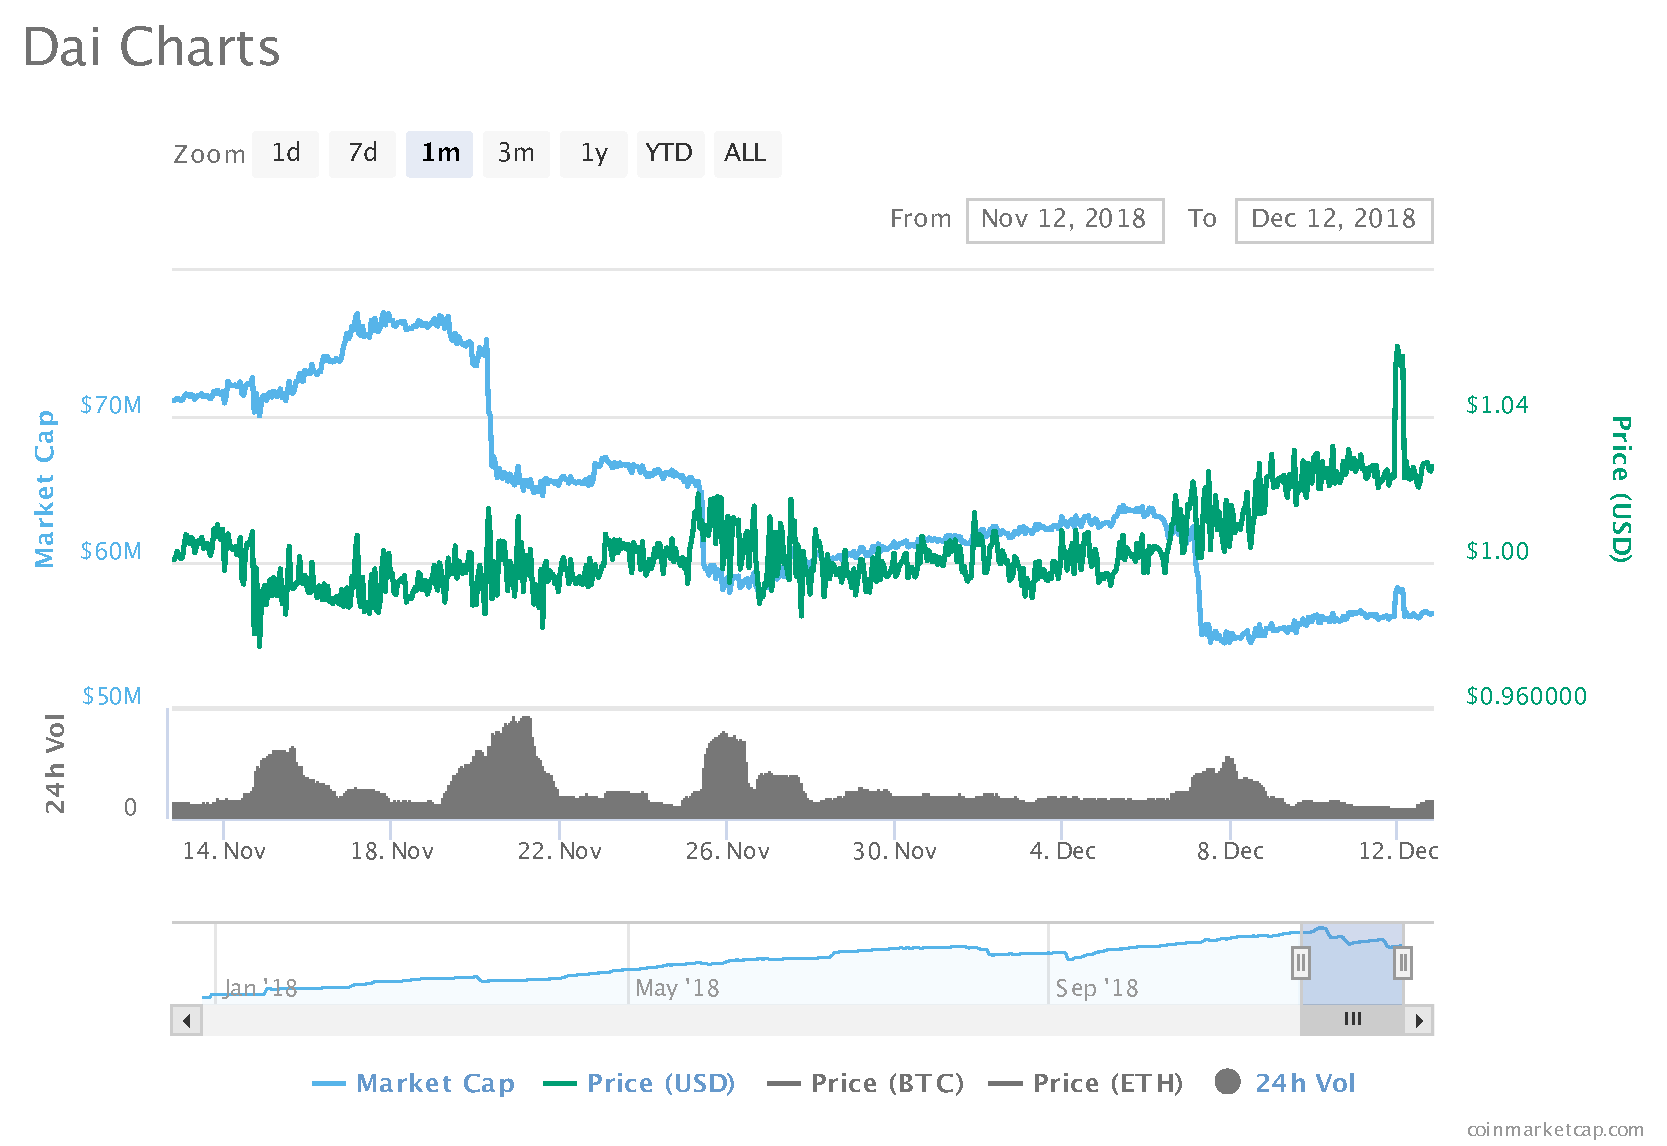
\includegraphics[width=\textwidth]{figures/dai_chart}
		\caption{}\label{fig:dai_chart}
	\end{subfigure}
	%
	\begin{subfigure}[b]{0.49\textwidth}
		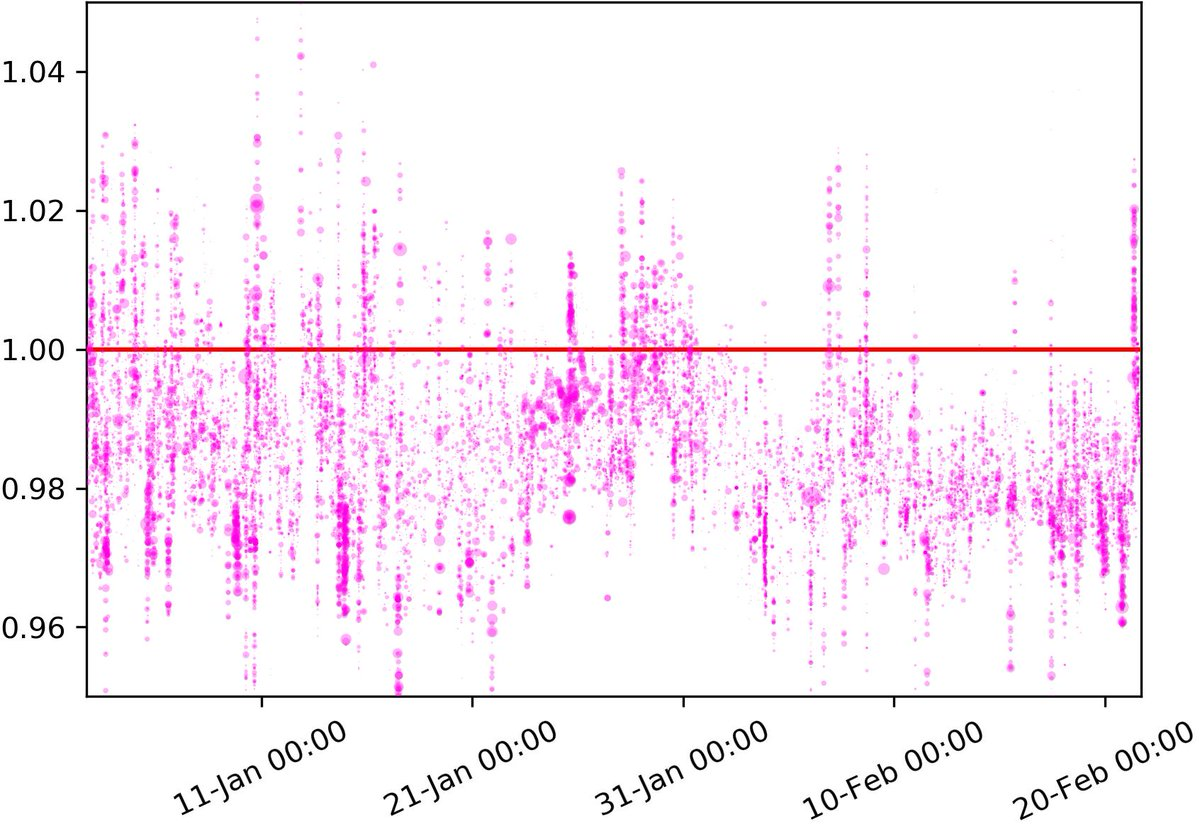
\includegraphics[width=\textwidth]{figures/dai_below_target}
		\caption{}\label{fig:dai_below_target}
	\end{subfigure}
	\caption{Model Results explain data from Dai market. (a) Dai deleveraging feedback in Nov-Dec 2018 (image from coinmarketcap). (b) Dai normally trades below target with spikes in price due to liquidations (image from dai.stablecoin.science).}\label{fig:real_liquidity}
\end{figure}

Since releasing the initial version of this paper in June 2019, massive liquidation events around Black Thursday in March 2020 provide additional strong evidence of deleveraging effects in the Dai market. Figure~\ref{fig:eth_mar20} depicts a $\sim 50\%$ ETH price cash on 12 Mar. 2020, which precipitated a cascade of cryptocurrency liquidations. Figure~\ref{fig:dai_mar20} depicts the price effects of these liquidations on Dai prices on DEXs. Speculators deleveraging during this event had to pay premiums of $\sim 10\%$ and face consistent premiums $>2\%$ weeks into the aftermath. 
Concurrently, Maker was affected by global mempool flooding on Ethereum. This additionally contributed to Dai liquidation auctions clearing at near zero prices, which may in fact have amplified the deleveraging feedback effects. Altogether, Dai traded at significant premiums over this time despite Maker being in a much riskier state in terms of collateral and liquidations.
See \cite{klagesmundt2020insights} and \cite{blocknative2020} for further discussion of this event.

\begin{figure}
	\centering
	\begin{subfigure}[b]{0.49\textwidth}
		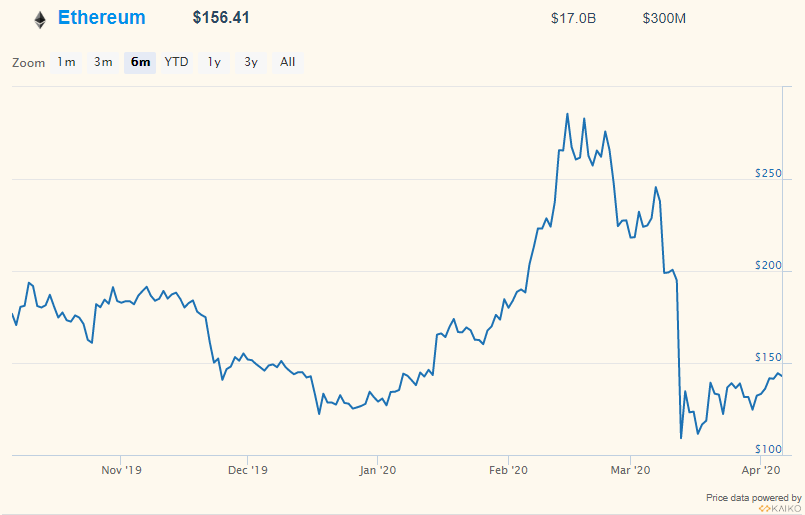
\includegraphics[width=\textwidth]{figures/ETH_prices_Mar2020_onchainfx}
		\caption{}\label{fig:eth_mar20}
	\end{subfigure}
	%
	\begin{subfigure}[b]{0.49\textwidth}
		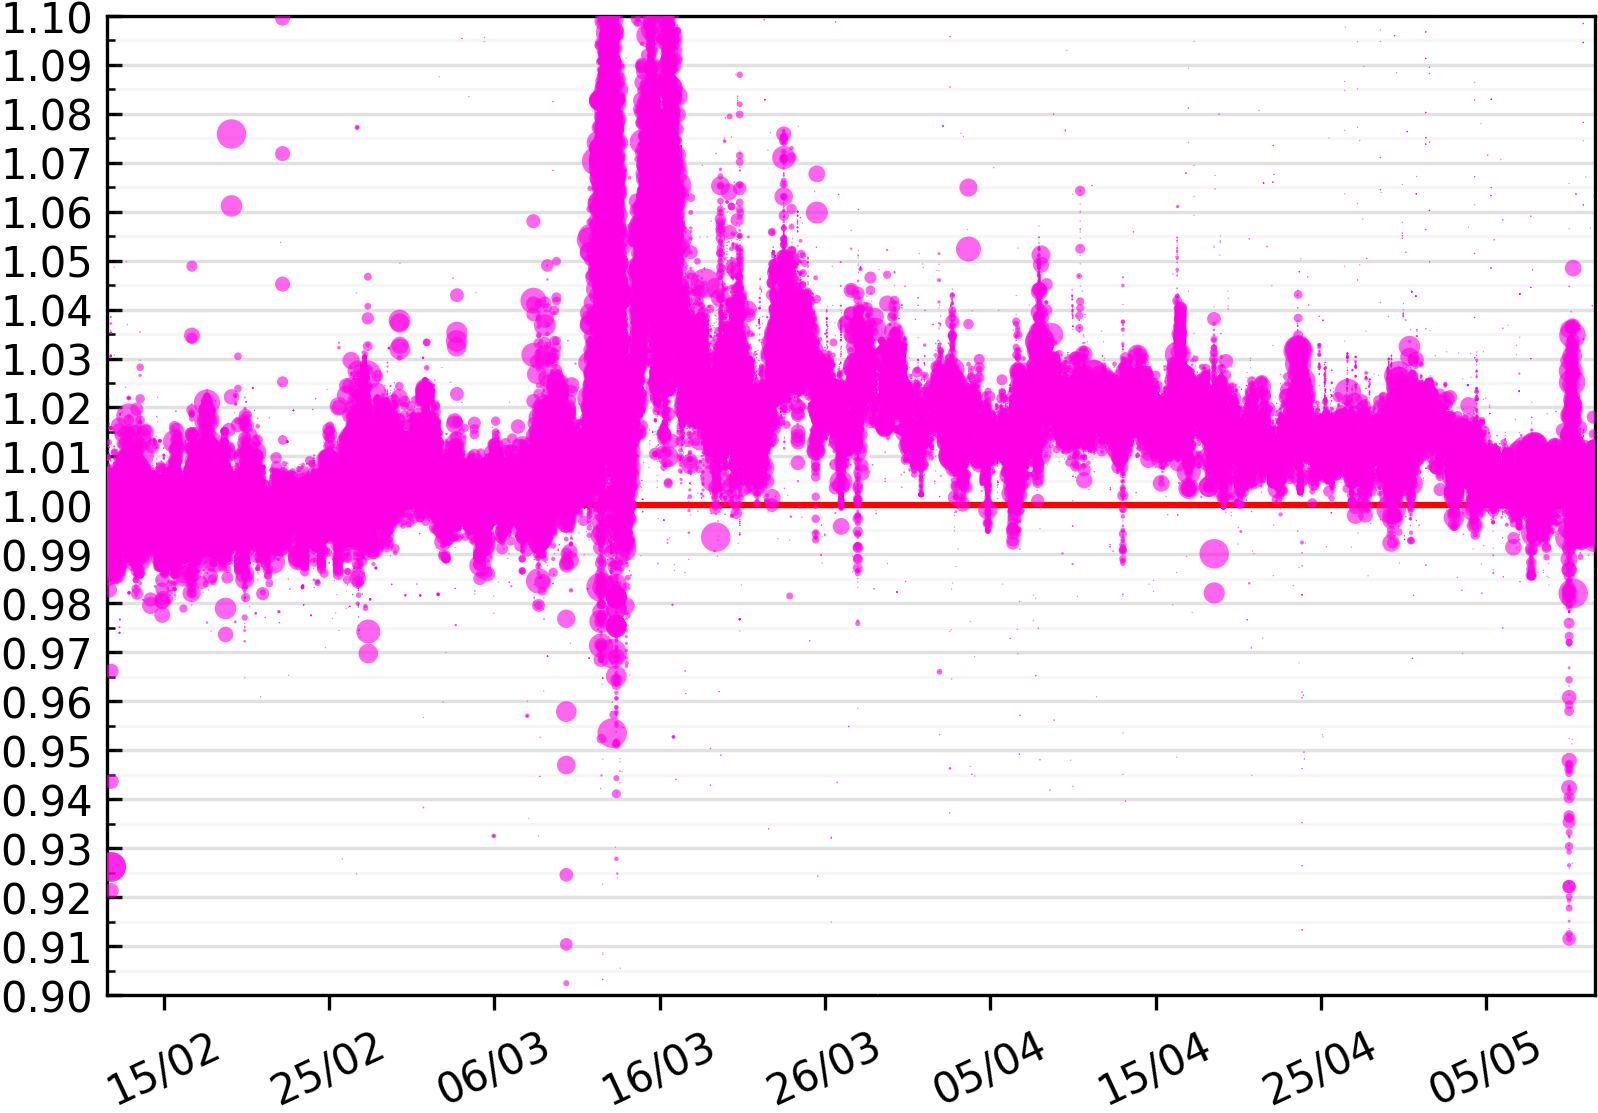
\includegraphics[width=\textwidth]{figures/ETHDAI-chart-90d}
		\caption{}\label{fig:dai_mar20}
	\end{subfigure}
	\caption{Black Thursday in March 2020. (a) $\sim 50\%$ ETH price crash (image from OnChainFX). (b) liquidation price effect on Dai DEX trades (image from dai.stablecoin.science).}\label{fig:mar20}
\end{figure}












%%%%%%%%%%%%%%%%%%%%%%%%%%%%%%%%%%%%%%%%%%%%%%%%%%%%%%%%%%%%%%%%%%%%%%%%%%%%%%%%%%%%%%%%%%%%%%%%%%%%%%%%%%
%%%%%%%%%%%%%%%%%%%%%%%%%%%%%%%%%%%%%%%%%%%%%%%%%%%%%%%%%%%%%%%%%%%%%%%%%%%%%%%%%%%%%%%%%%%%%%%%%%%%%%%%%%
%%%%%%%%%%%%%%%%%%%%%%%%%%%%%%%%%%%%%%%%%%%%%%%%%%%%%%%%%%%%%%%%%%%%%%%%%%%%%%%%%%%%%%%%%%%%%%%%%%%%%%%%%%
\section{Stability results}\label{sec:stable_v_unstable}

We now characterize stable price dynamics of DStablecoins when the leverage constraint is non-binding. For this section, we make the following simplifications to focus on speculator behavior:
\begin{itemize}
	\item The market has fixed dollar demand at each $t$: $w^D_t \mathcal{A}_t = \mathcal{D}$. This is consistent with the stablecoin holder having unit-elastic demand, or having an exogenous constraint to put a fixed amount of wealth in the stable asset.
	\item Speculator's expected Ether return is constant $r_t = \hat r>1$. This means they always want to fully participate in the market and is consistent with $\gamma=0$.
\end{itemize}
This amounts to setting $x = \mathcal{D}$ and $y=-\mathcal{L}$. Now the DStablecoin market clearing price is
$p^D_t = \frac{\mathcal{D}}{\mathcal{L}_t}.$
The leverage constraint (assuming $\mathcal{L} + \Delta > 0$) becomes
$$-\beta\Delta^2 + \Delta(\tilde\lambda(z+\mathcal{D}) - 2\beta\mathcal{L}) + \mathcal{L}(\tilde\lambda z - 2\beta - \beta\mathcal{L}) \geq 0.$$

The speculator's maximization objective becomes
$\hat r\Delta \frac{\mathcal{D}}{\mathcal{L}+\Delta} - \Delta,$
which gives
$$\Delta^* = -\mathcal{L} + \sqrt{\mathcal{L}\mathcal{D}\hat r}.$$

While we prove a stability result in this simplified setting, we believe the results can be extended beyond the assumption of constant unit-elastic demand.



\subsection{Stability if leverage constraint is non-binding}
\begin{proposition}\label{prop:stable1}
	Assume $w_t^D \mathcal{A}_t = \mathcal{D}$ (DStablecoin dollar demand) and $r_t = \hat r$ (speculator's expected Ether return) remain constant. If the leverage constraint is inactive at time $t$, then the DStablecoin return is
	$$\frac{p^D_t}{p^D_{t-1}} = \sqrt{\frac{\mathcal{L}}{\mathcal{D}\hat r}}.$$
\end{proposition}

\begin{center} \hyperlink{pf:stable1}{\texttt{[Link to Proof]}} \end{center}


Supposing that $\mathcal{D}\approx \mathcal{L}$ (i.e., the previous price was close to the \$1 target) and the constraint is inactive, Prop.~\ref{prop:stable1} tells us that the DStablecoin behaves stably like the payment of a coupon on a bond.

Consider estimators for DStablecoin log returns $\bar \mu_t$ and volatility $\bar \sigma_t$ computed in a similar way to Ether expectations in Eq.~\ref{eq:expectations}. When the leverage constraint is non-binding, DStablecoin log returns remain $\bar \mu_t \approx 0$, the contribution to volatility at time $t$ is $\ln \frac{p_t^D}{p_{t-1}^D} - \bar \mu_t \approx 0$, and the DStablecoin tends toward a steady state with stable price and zero variability. The next theorem formalizes this result to describe stable dynamics of price and the volatility estimator under the condition that the system doesn't breach the speculator's leverage threshold.

\begin{theorem}\label{prop:stable2}
	Assume $w_t^D \mathcal{A}_t = \mathcal{D}$ (DStablecoin demand) and $r_t = \hat r$ (speculator's expected Ether return) remain constant. Let $\mathcal{L}_0=\mathcal{D}$ and $\bar \mu_0, \bar \sigma_0$ be given. If the leverage constraint remains inactive through time $t$, then
	$$\mathcal{L}_t = \mathcal{D}\hat{r}^{\frac{2^t-1}{2^t}},
	%\hspace{1cm} \ln \frac{p^D_t}{p^D_{t-1}} = -2^{-t} \ln \hat r$$
	\hspace{1cm} \bar \mu_t = \begin{cases}
	(1-\delta)^t \bar \mu_0 - \delta \frac{(1-\delta)^t-2^{-t}}{2(1-\delta)-1} \ln \hat r, & \text{ if } \delta \neq 1/2 \\
	2^{-t}\Big( \bar \mu_0 - \frac{1}{2} t \ln \hat r \Big), & \text{ if } \delta = 1/2
	\end{cases}$$
	$$\bar\sigma_t^2 = \begin{cases}
	\sum_{k=1}^t (1-\delta)^{t-k}\delta \Big( (1-\delta)^k \bar \mu_0 - \frac{(1-\delta)^k -2^{-k+1}(1-\delta)}{2(1-\delta)-1}\ln \hat r \Big)^2 + (1-\delta)^t\bar\sigma_0^2, & \text{ if } \delta \neq 1/2 \\
	2^{-t} \sum_{k=1}^t 2^{-k-1} \Big( (k/2-1)\ln \hat r - \bar \mu_0\Big)^2 + 2^{-t} \bar\sigma_0^2, & \text{ if } \delta=1/2
	\end{cases}$$
	Further, assuming the constraint continues to be inactive and that $\delta \leq \frac{1}{2}$, the system converges exponentially to the steady state
	$\mathcal{L}_t \rightarrow \mathcal{D}\hat r$,
	$\bar \mu_t \rightarrow 0$,
	$\bar\sigma_t^2 \rightarrow 0$.
\end{theorem}

\begin{center} \hyperlink{pf:stable2}{\texttt{[Link to Proof]}} \end{center}



Notice that if the leverage constraint in the system is reached, we can still treat the system as a reset of $\bar\mu_0$ and $\bar\sigma_0$ when we reach a point at which the constraint is no longer binding. While the system subsequently remains without a binding constraint, we again converge to a steady state starting from the new initial conditions.


\paragraph{Interest rates and trading below \$1.}
A consequence of Theorem~\ref{prop:stable2} is that the DStablecoin will trade below target during times in which Ether expectations are high. This is empirically seen in Figure~\ref{fig:dai_below_target}. An interest rate charged to speculators can balance the market (the `stability fee' in Dai). This can temper expectations by effectively reducing $r$ in Theorem~\ref{prop:stable2}. In the stable steady state, setting the interest rate to offset the average expected ETH return will achieve the price target. However, this is practically difficult as $r$ changes over time and is difficult to measure accurately. It also depends on holding periods of speculators. It is an open question how to target these fees in a way that maintains long-term stability.




\subsection{Instability if leverage constraint is binding}\label{sec:instability}
When the speculator's leverage constraint is binding, DStablecoin price behavior can be more extreme. We argue informally that this can lead to high volatility in our model. The probability distribution for the leverage constraint to be binding in the next step has a kink at the boundary of the leverage constraint. In particular, it becomes increasingly likely that the leverage constraint is binding in a subsequent step due to deleveraging effects described previously. Note that feedback of large liquidations on Ether price, if added to the model, will add to this effect.

We show such instability computationally in Figure~\ref{fig:hist_constraint_returns} in simulation results. In this figure, the shape of the inactive histogram reflects the speculator's willingness to sell at a slight discount when the leverage constraint is non-binding due to the constant $\hat r$ assumption.

We relax this assumption in Figure~\ref{fig:hist_vol_learning_rate}, which shows the effects on volatility of different speculator memory parameters. This figure is a heat map/2D histogram. A histogram over $y$-values is depicted in the third dimension (color: light=high density, dark=low density) for each $x$-value. Each histogram depicts realized volatilities across 10k simulation paths using the simulation setup introduced in the next section and the given memory parameter ($x$-value). Horizontal lines depict selected percentiles in these histograms. The dotted line depicts the historical level of Ether volatility for comparison.

In Figure~\ref{fig:hist_vol_learning_rate}, volatility is bounded away from 0 even in non-binding leverage constraint scenarios; the distance increases with the memory parameter. This happens because $r$ updates faster with a higher memory parameter. As the speculator's objective then changes at each step, the steady state itself changes. Thus we expect some nonzero volatility, although it remains low in most cases.

In not-so-rare cases, however, volatility can be on the order of magnitude of actual Ether volatility in these simulations. As seen in Figure~\ref{fig:vol_risk_mgmt}, this result is robust to a wide range of choices for the speculator's risk constraint. This suggests that DStablecoins perform well in median cases, but are subject to heavy tailed volatility.


\begin{figure}
	\centering
	\begin{subfigure}[b]{0.49\textwidth}
		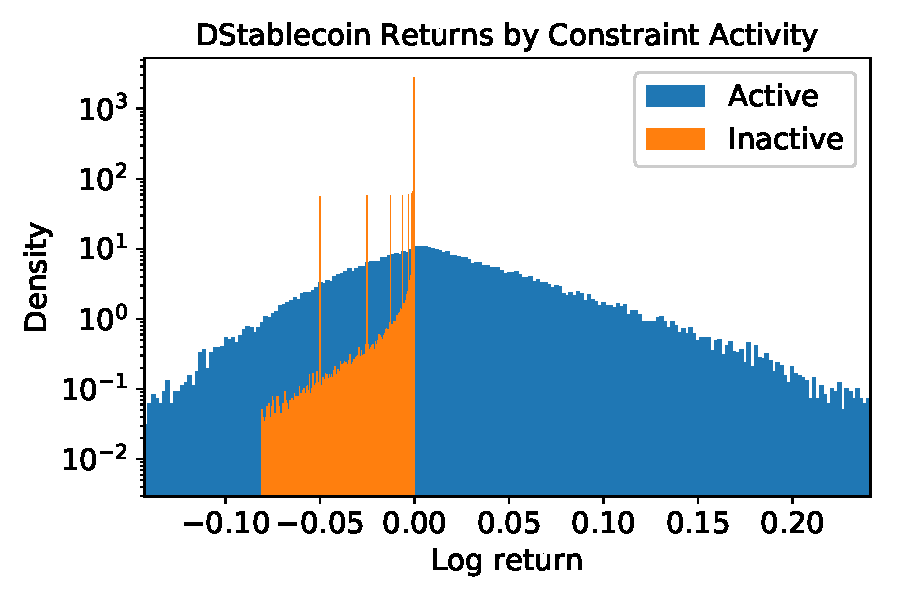
\includegraphics[width=\textwidth]{figures/hist_constraint_returns}
		\caption{Histogram of DStablecoin returns when leverage constraint is binding vs. non-binding with constant $\hat r$.}\label{fig:hist_constraint_returns}
	\end{subfigure}
	\begin{subfigure}[b]{0.49\textwidth}
		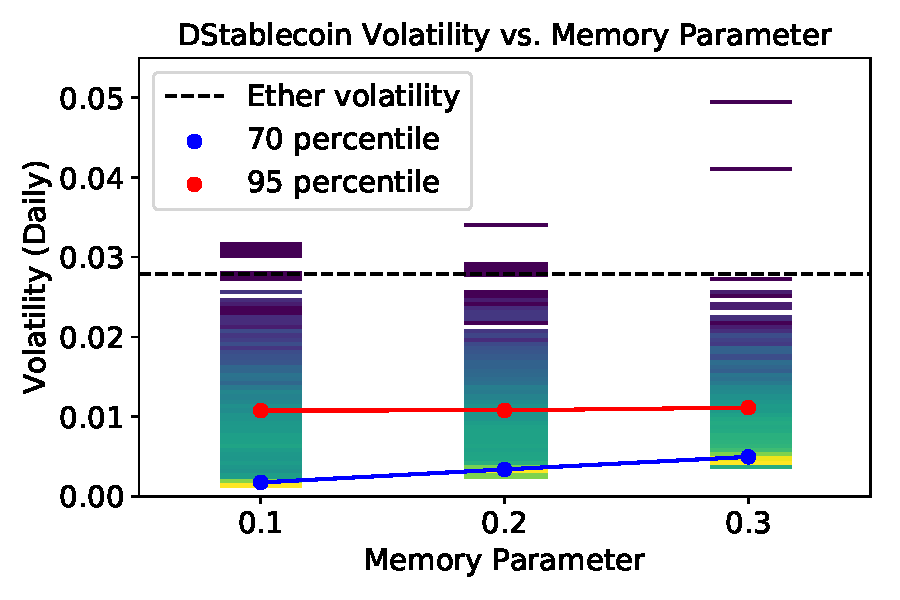
\includegraphics[width=\textwidth]{figures/hist_vol_learning_rate}
		\caption{Heat map of volatility under different speculator $\gamma=\delta$ memory parameters.}\label{fig:hist_vol_learning_rate}
	\end{subfigure}
	\caption{DStablecoin volatility, 10k simulation paths of length 1000.}
\end{figure}




